\chapter{Introduction}\label{ch:introduction}


\instructionsintroduction



\section{High-throughput data and the system biology}

Molecular biology has dominated the biology research in the past century with exciting progresses: the discovery of DNA and its structure, the revelation of the central dogma, the disclosure of message RNA. Accompanied by the proliferate developments in biotechnology like the recombinant DNA technology, the polymerase chain reaction, and the DNA sequencing, these processes of replication, transcription, and translation have been extensively studied. Due to the technological limitations, the molecular biologist has taken a reductionist approach to study a handful of genes or even single gene in isolation to uncover their connections with the observable characters of an organism (phenotype). However, ever since the discovery of the complex regulation mechanism of Lac operon \cite{Jacob1961}, there has been a growing understanding that an organism is a complex system whose characteristics and behaviors are often driven by complicated interactions among its components instead of single gene.  Yet, the early efforts were hampered by the lack of experimental technologies to harvest the data required to study an organism at the system level.


Heralding the coming high-throughput era, two technological breakthroughs in 90s dramatically improved our data collection ability, and revolutionized the molecular biology research. First, automated DNA sequencers emerged and soon reached genome-scale sequencing \cite{Fleischmann1995}, enabling, for the first time, the study of the complete genetic material and the discovery of the full gene universe of a species. This is followed by the development of the microarray technologies \cite{Pease1994, Schena1995} that was utilized first to study the gene expression at genome-scale \cite{Davis1997}, and later to generate additional `omics' data types \cite{Blat1999, Uetz2000}. Due to their unprecedented ability, accompanied by the swift developments of required computational tools, these technologies were broadly adopted in biology researches, and shortly in a scaled-up settings \cite{Su2002,Su2004}. The availability of various types of data for an organism at genome-scale finally expedited the emergence of system biology as an approach to biological research.  System level models of interacting components are constructed in order to provide insights into the function and control of biological systems that are not apparent from studying the individual component, and in turn, to generate experimentally verifiable hypotheses that deepen our understanding of those systems \cite{Ideker2001, Palsson2002}. The advance in system biology commands ever more comprehensive data set. However the amount of data generated by individual experiment is physically constrained by the number of biological samples tested, whereas a colossal volume of gene expression experiments are publicly available but largely remain underutilized. The research presented in this dissertation aims on bridging this gap by developing a methodology to construct comprehensive organism-specific expression compendia through a direct integration of publicly available experiment data.



\section{Microarrays and data preprocessing}

Fundamentally hybridization based, the microarray technology has its root in Southern blotting, where fragmented DNA attached to a substrate are probed with a known DNA sequence. Although the earliest approach that resembles microarray appeared in 80s \cite{Augenlicht1982}, it is not until large amount of sequences became available following the advances in the automated sequencing technology that a microarray capable of probing thousands of genes' expression simultaneously has become possible. And the first genome-scale microarray for \textit{Saccharomyces   cerevisiae} \cite{Davis1997} appeared shortly after its complete genome sequence was released \cite{Goffeau1996}. With its unprecedented ability, microarray has quickly become an indispensable technology to quantify global gene expressions.


There are different microarray platforms for measuring gene expression, such as Affymetrix, Agilent, Nimblegen, or in-house microarrays \cite{Sasik2004}. They can be categorized according to the number of samples that can be hybridized simultaneous on a chip. \textit{Two-channel microarrays} or \textit{dual-channel microarrays} are typically hybridized with cDNA prepared from two samples and labeled with two different fluorophores (commonly Cy3 with green color and Cy5 with red color). Relative intensities of each fluorophore (color channel) are used to calculate ratios representing gene expression changes to identify up-regulated and down-regulated genes between samples. Typical example of dual-channel microarrays are cDNA arrays whose probes are cDNAs synthesized from mRNAs. In \textit{one-channel microarrays} or \textit{single-channel   microarrays}, only one sample is hybridized to a chip generating intensity data for each probe or probeset. However these intensities do not reflect the absolute abundance levels of a gene but rather the relative ones when compared to other samples or conditions processed in the same experiment, as the experimental protocol and batch-specific biases render a direct comparison of gene's intensities of same platform origin across experiments uninformative. Affymetrix ``Gene Chip'', the most popular one of such platforms due to its high accuracy and precision \cite{Irizarry2005}, is used as an example to discuss the issues related to this type of arrays.


%% \textbf{Microarray data processing}
Microarray data are very noisy.  There are many sources of systematic variation in microarray experiments that affect the measured gene expression levels, such as, heat and light sensitivity, dye labeling and detection efficiency, and unequal quantities of starting RNA, etc \cite{Kerr2001,Zakharkin2005}. It is crucial to apply normalization procedures on raw expression intensities to remove systematic bias arising from the variations in the microarray technology rather than from biological differences between samples  \cite{Quackenbush2002}. Various methods have been developed for this purpose, and most are platform dependent.

For cDNA microarray, the log-ratios calculated from the per-channel intensities from the same spot (probe) theoretically negate most of the systematic noises related to manufacture variations, such as, spot effect, print-tip effect, etc. However, often there exists intensity dependent artifacts in the obtained log-ratios which can be visualized in a MA plot \cite{Yang2002}. Locally weighted linear regression (LOWESS) analysis \cite{Cleveland1979} first proposed by Yang \textit{et al.} \cite{Yang2002} has been shown to successfully remove such artifacts, and became the most widely used normalization method for cDNA microarray. This method was later replaced by LOESS (LOcal regrESSion) which is more flexible albeit computationally more intensive.


For single-channel microarray, such as, Affymetrix platform, a desirable normalization method needs to remove all variations of non-biological origin across arrays, as each array generates relative gene expression intensities for one sample only, whereas gene expressions of different samples (produced on different arrays) must be made comparable to observe true variations originated from biological differences between samples. Among the large number of methods developed for the popular Affymetrix platform, a global quantile normalization \cite{Bolstad2003,Irizarry2003a} coupled with medial polish summarization \cite{Irizarry2003}, combinedly known as robust multi-array average (RMA) method, has been shown to outperform other methods \cite{Irizarry2006} providing better precision even with few biological replicates.  It soon became the \textit{de facto} standard normalization method for this platform.









\section{Gene expression compendium}


As microarray become an indispensable technology for studying gene expression, large amount of data has been generated. To promote data sharing, scientific journals generally require the deposit of these high-throughput experiments in public databases, such as Gene Expression Omnibus (GEO) \cite{Barrett2011} or ArrayExpress \cite{Parkinson2009}, upon publication. These databases are an extremely rich source of information, containing freely accessible data for thousands of experiments and a multitude of different organisms, and in theory provide an opportunity to analyze gene expression of a particular species at a global level \cite{Ideker2001}. Additionally, they hold the potential to expand the scope of any smaller scale study: mining the existing information offers molecular biologists the possibility to view their own dedicated experiments and analysis in light of what is already available.






\subsection{Data integration issues}

However, the opportunity of combining all public experiments for a single organism has not been explored due to two practical issues, data heterogeneity and data representation heterogeneity. First, microarray data are inherently highly heterogeneous. Data sets originate from different experimenters or labs and microarrays do not constitute a uniform technology. Even for data generated on one platform, protocols for sample preparation, labeling, hybridization, and scanning can vary greatly across labs and even studies, deteriorating the data compatibility \cite{Bammler2005, Irizarry2005}. The consistency among data generated on different platforms is even worse due to the probe design and manufacture variations \cite{Sasik2004, Draghici2006}. Moreover, the aforementioned platform-dependency of pre-processing methods further lowers the data coherence, as often, different studies employ different methods \cite{Irizarry2005, Shi2006, Stafford2007}. Second, although community standards specifying the mandatory minimal experimental information accompanying each dataset (e.g., MIAME \cite{Brazma2001}) have been long established, the lack of the requirements \cite{Brazma2009} imposed regarding the format of the platform descriptions and the expression measurements, as well as the degree of preprocessing done on these values further complicates the matter of experiment integration from a practical point of view. 


\subsection{Existing compendium construction efforts}

Despite such difficulties, several initiatives exist to actively build expression compendia from public resources. Reviewed in Fierro \textit{et al.} \cite{Fierro2008}, the existing compendia took two different approaches to alleviate the aforementioned data integration issues: directly integrating data across experiments albeit limited by only those generated on a single-platform \cite{Faith2008, Hruz2008}, or combining results of individual experiment through meta-analysis to avoid direct data integration across experiments \cite{Rhodes2007, Pan2007, Elfilali2006,   Kapushesky2010, Culhane2012}.



Meta-analysis is capable of combining data from different experiments across variant platforms, albeit in an indirect manner. It is generally a two step analysis: one first applies the desired analysis procedure (e.g., identifying differentially expressed genes, clustering gene expression profiles, etc.) on each single data set within the compendium separately, and subsequently combines the derived results. These compendia are often topic-specific, collecting all publicly available experimental information related to a subject matter of interest.  ITTACA \cite{Elfilali2006} and ONCOMINE \cite{Rhodes2007}, for instance, focus on cancer in human; Gene Aging Nexus \cite{Pan2007} on aging in several species; GeneSigDB for gene signatures of cancer and related diseases \cite{Culhane2012}. Exceptionally, the ATLAS \cite{Kapushesky2010} initiative from ArrayExpress provides gene expression meta-analysis data sets for several species.  However, containing only 400 experiments over all species in total and biased towards several eukaryotic model organisms, it is still far from comprehensive.



Alternatively, the direct integration approach removes data heterogeneity by applying normalization method across studies, then merges the results together to form one expression data set. Ideally, all data publicly available for a species could be integrated into one comprehensive compendium. Due to the aforementioned issues, the existing ones, however, focus on gathering only the data generated by single platform, for instance, M$^{\textrm{3D}}$ \cite{Faith2008} or the commercial Genevestigator \cite{Hruz2008}. The Affymetrix platform is often chosen as the target platform, as they are the most widely used ones due to their robustness and high reproducibility \cite{Bammler2005, Irizarry2005}. The single-channel nature of the Affymetrix platform and the use of proprietary file formats to report platform information and expression measurements avoid the data representation heterogeneity that plagues the data generated by many other platforms, and make the data collection task straightforward. Combining data from a single platform makes the in-between experiment normalization and probe mapping relatively straightforward, so that the quantitative measures of gene expression can be analyzed directly across experiments. For eukaryotic model organisms, such a single-platform approach works well as the compendium based on Affymetrix chips can achieve a broad scope on experimental condition due to the platforms popularity. For instance, Lukk \textit{et al.} \cite{Lukk2010} created a comprehensive data set for human containing 5372 microarrays representing 369 different cell and tissue types, disease states and cell lines. For prokaryote, however, the single-platform constraint severely circumscribes the scope of the compendium created due to the lack of such a dominate platform. Even for a widely studied model organism, such as {\it E. coli}, the most  popular platform `Affymetrix GeneChip E. coli Genome 2.0 Array' is used in less  then one thirds of all publicly available experiments. When considering only one platform, a significant portion of data is missed out  on.  A novel approach that can integrate data of different platform origin is highly desirable.



When combining data from multiple experiments that address a set of related research questions, both meta-analysis and direct data integration approaches enjoy the benefit of higher statistical power and more robust inference due to the increased number of samples in the combined data set and the reduced effect of study-specific biases \cite{Sutton2001, Xu2005, Warnat2005}. However, when compared to direct data integration, meta-analysis approach has several disadvantages. First, the meta-analysis approach can only generalize those biological findings which are statistically significant in a high enough number of individual studies.  This results a great lose of information, and consequently leads to high false-negative rates \cite{Lazar2012, Xu2008}. It has been observed that when compare meta-analysis and direct analysis of integrated data for differential expressed gene retrieval, taking the results obtained by the analysis of a single experiments as a reference, direct analysis of multiple experiments detects more differentially expressed genes while indirect analysis tend to result in a more restricted gene list which corresponds \textit{grosso modo} to the intersection of the sets of differentially expressed genes obtained by each of the single experiments \cite{Fierro2008}. On the contrary, all the data are retained in the direct integration approach. New discovery can be generated when the combined data are analyzed together. Indeed, Warnat \textit{et al.} \cite{Warnat2005} shows that direct integration reveals novel genes that is otherwise missed in single-set analysis, and the classifier incorporating those genes shows high predictive power and improved generalization performance. Second, the compendium based on meta-analysis are limited by the predefined functionalities provided by the system, hence lack of flexibility to incorporate new analysis.   The ones created by direct integration, however, retain actual expression values, hence the compendia can be readily analyzed by the existing and potential methods.  This greatly broadens the scope of the utility of the compendium. For example, the \textit{E. coli} compendium of M$^{\textrm{3D}}$ \cite{Faith2008}, which is originally created to study transcriptional regulation in this species, has been applied to benchmark network inference algorithm \cite{Marbach2012}, to discover conserved biclusters across multiple species \cite{Kacmarczyk2011}, and to study chromosome conformation alternations under different physiological conditions \cite{Ma2013}, etc.







\section{Objective and Overview of the dissertation}

Apparently, there exists a dilemma: on one hand the amount of data generated by individual experiment is physically constrained by the number of biological samples available, whereas on the other hand a colossal volume of diverse gene expression experiments are publicly available but largely remain underutilized. The main goal of this thesis aims to tackle this issue by creating a method that constructs an organism-specific cross-platform gene expression compendium through direct data integration, and developing systems and tools that facilitate the access and utility of such compendium. Having the advantage of direct integration, while not being limited to a single platform, such compendium can provide an unprecedentedly broad coverage on variant experimental conditions and over diverse biological samples. To achieve the first goal, we carefully analyzed the issues that prevent direct data integration across platforms, then derived various specific strategies to handle those issues and conceived a three-step methodology for cross-platform compendium creation, and at last, developed a system incorporating the methodology to facilitate compendium creation and, vitally, the continuous curation to keep it up-to-date. The second objective focuses on identifying straightforward data analysis functionalities compatible with the type of data in the compendium, and developing an user-friendly system to facilitate the utility of data by a broader range of audiences. At last, we aim to expend the applicability of our methodology to eukaryotes by upgrading the existing systems with extra functionalities to handle the complexity of such species. This is demonstrated by creating a comprehensive \textit{Zea mays} compendium.



\begin{figure}
  \centering
  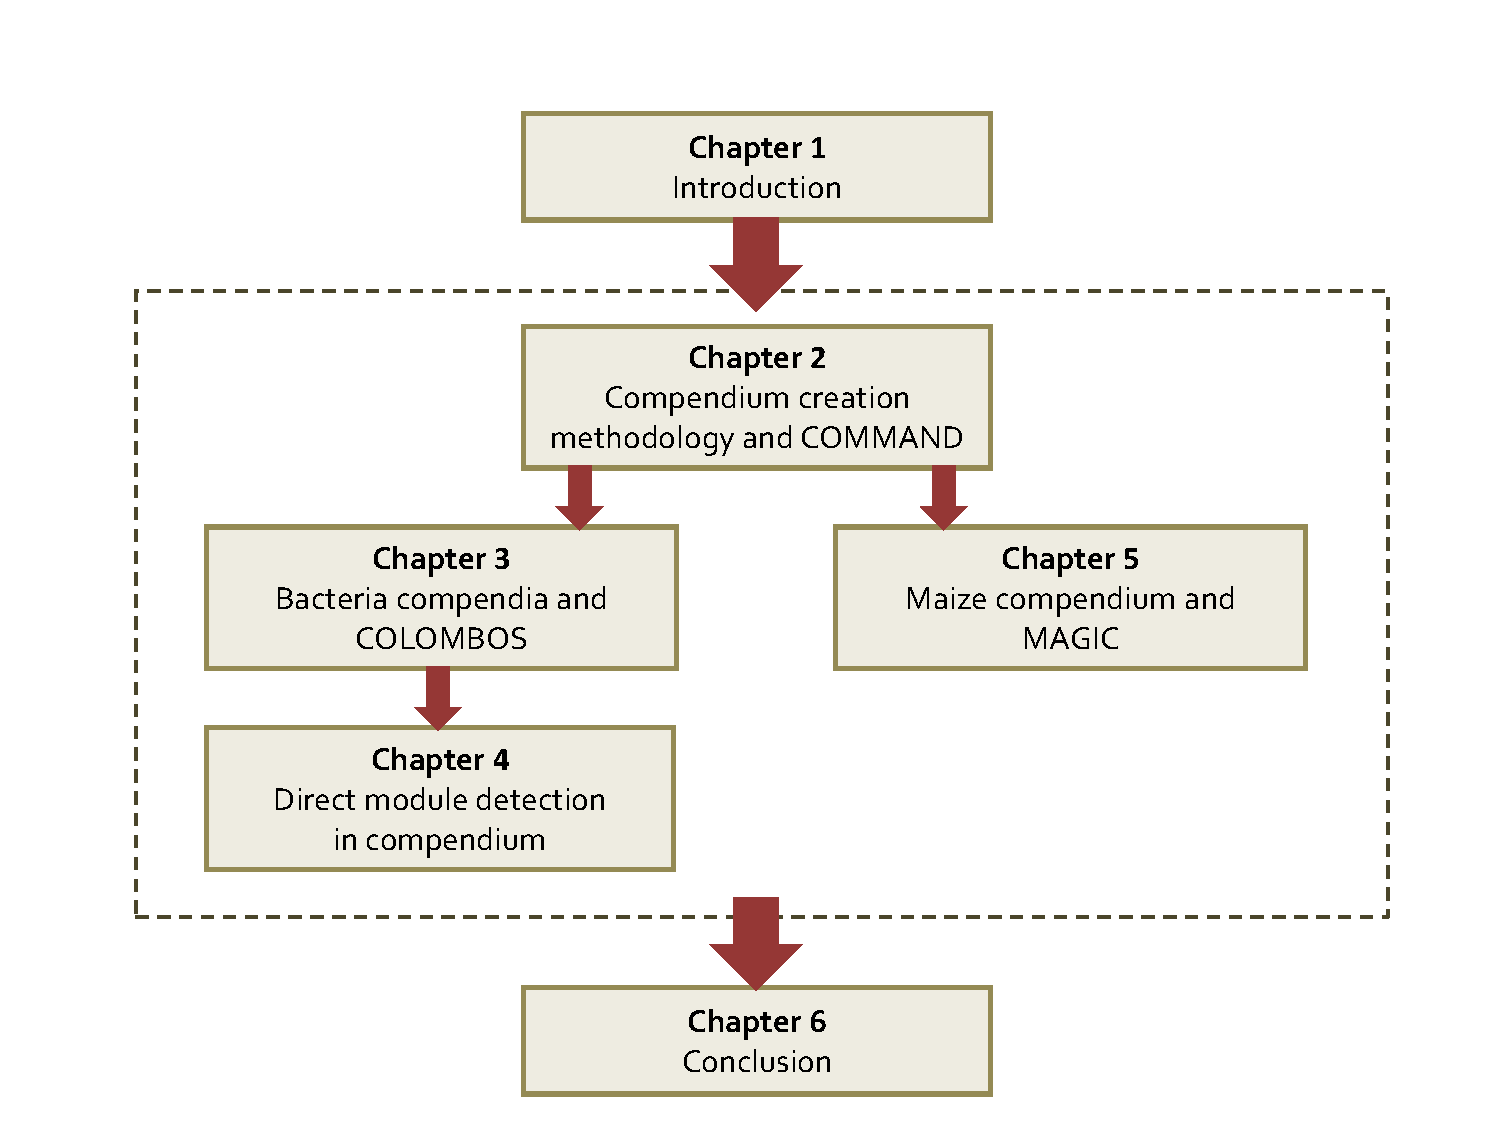
\includegraphics[trim=0cm 0cm 0cm 1cm, clip=true, width=1\textwidth]
                  {thesis_structure.pdf}
  \caption[Organization of the dissertation]{
     \textbf{Organization of the dissertation}}. 
  \label{fig:intro_overview}
\end{figure} 

The topics covered in this thesis are centered around this organism-specific cross-platform expression compendium (Figure \ref{fig:intro_overview}).  Chapter \ref{ch:command} describes the development of a methodology that enables the creation of an organism-specific cross-platform expression compendium. We first thoroughly investigated the issues involved in creating cross-platform compendium, including, the data representation heterogeneity, particularly for those related to the data generated on dual-channel microarrays, the lack of standards to specify experimental meta-data, and the sources of data inconsistency across experiments and platforms. Based on our study, we conceived a compendium creation methodology containing three major steps: data collection, annotation, and homogenization, each of which targets one specific issue identified. To reduce the complexity involved in compendium creation and facilitate the maintenance of existing ones, we then developed a web system that provides user friendly interfaces to guide user through various steps of compendium creation. The methodology lays the foundation of this research work. In Chapter \ref{ch:colombos}, three such cross-platform compendia for bacterial model organisms (\textit{Escherichia coli}, \textit{Bacillus   subtilis}, and \textit{Salmonella enterica} serovar Typhimurium) are presented together with a web access portal COLOMBOS that incorporates a suite of intuitive tools for data exploration, analysis and visualization and provides easy-of-use access to these compendia. The utility of both the compendia and the web portal is demonstrated in a case study, in which COLOMBOS analysis tools are employed to identify novel targets for \textit{E. coli} transcription factor FUR (Ferric Uptake Regulation) based on their expression similarity to that of the known FUR targets across a range of diverse conditions in \textit{E. coli} compendium. Chapter \ref{ch:distiller} further showcased the utility of the compendium in the application of query driven condition dependent co-expression module discovery. Two web services, DISTILLER \cite{Lemmens2009} and COLOMBOS \cite{Engelen2011}, are recruited to explore \textit{E. coli} compendium and identify such modules for query gene \textit{sodA}. We demonstrate that the complementarity between the results obtained by each approach well reflects the complementarity nature of these two approaches, and the choice of the method depends on the nature of the biological questions to be answered. Chapter \ref{ch:magic} describes our attempt to create a cross-platform expression compendium for eukaryotic organisms utilizing the methodology. Here, we specifically address two issues: platform probe heterogeneity due to the lack of the complete genome sequence, and precise biological sample annotation that manifests the abundant genetic repository (breeding lines) of maize species and its complex life style (development stage) and structure (tissue). At the end, the main achievements of this PhD study are summarized in Chapter \ref{ch:conclusion} followed by some perspectives for future research.










% glossary

\glossary{name=GEO, description=Gene Expression Omnibus}
\glossary{name=EBI, description=European Bioinformatics Institute}
\glossary{name=NCBI, description=National Center for Biotechnology Information}


\glossary{name=COLOMBOS, description=Collection of Microarrays for Bacterial 
Organisms}
\glossary{name=DISTILLER, description=Data Integration System to Identify Links 
in Expression Regulation}
\glossary{name=ViTraM, description=VIsualization of TRAnscriptional Modules}
\glossary{name=EcoCyc, description=Encyclopedia of \textit{Escherichia coli} 
K-12 Genes and Metabolism}
\glossary{name=BioCyc, description=Pathway/Genome Databases and Pathway Tools 
Software}
\glossary{name=MaizeGDB, description=Maize Genetics and Genomics Database} 
\glossary{name=PLEXdb, description=Plant Expression Database}
\glossary{name=CORNET, description=CORrelation NETworks}
\glossary{name=BLAST, description=Basic Local Alignment Search Tool}


\glossary{name=PSSM, description=Position Specific Scoring Matrices}
\glossary{name=ChIP, description=Chromatin Immunoprecipitation}
\glossary{name=NGS, description=next generation sequencing}


\glossary{name=DNA, description=deoxyribonucleic acid}
\glossary{name=cDNA, description=complementary deoxyribonucleic acid}
\glossary{name=RNA, description=ribonucleic acid}
\glossary{name=UTR, description=untranslated region}


\glossary{name=iPOP, description=integrative personal omics profile}
\glossary{name=FGS, description=Filtered Gene Set}


\glossary{name=SOFT, description=Simple Omnibus Format in Text}
\glossary{name=GPR, description=GenePix Results format}
%\glossary{name=CEL, description=}
\glossary{name=CDF, description=Chip Description File}
\glossary{name=GPR, description=GenePix Results}
\glossary{name=IDF, description=Investigation Description Format file}
\glossary{name=SDRF, description=Sample and Data Relationship Format file}
\glossary{name=ADF, description=Array Design Format file}
\glossary{name=MAGE-TAB, description=MicroArray Gene Expression Tabular}
\glossary{name=MGED, description=Microarray Gene Expression Databases}
\glossary{name=MIAME, description=Minimum Information About A Microarray 
Experiment}




% nomenclature

\nomenclature{Compendium}{Essentially an expression (log-ratio) value matrix, 
whose rows correspond to the known genes and columns correspond to sample 
contrasts}

\nomenclature{Sub-compendium}{A subset of compendium containing contrasts 
sharing certain properties of interests, e.g., contrasts in which the gene 
expression profiles of different tissues are compared}

\nomenclature{Sample contrast}{Where the expression values of genes from two 
biological samples, one set at the test and the other reference, are compared 
and the expression variations between samples are represented as log ratio}

\nomenclature{Coexpression}{Genes' coherent expression responses to 
certain alterations in the organism's intra- or extracellular environment}

\nomenclature{Coexpression Module}{A combined set of genes and condition 
contrasts, where the coexpression pattern appears}

\nomenclature{Homogenization}{Our methodology to convert raw 
intensity expression values from individual biological sample into expression 
log-ratios between two different biological samples paired as a contrast so 
that they are comparable across different microarray platforms and experiments}

\nomenclature{Coregulation}{A phenomenon that genes are regulated by common 
transcription factor(s)}

\nomenclature{Frequent itemset mining}{A data mining technology tries to 
extract information about a set of items that occurs together frequently}

\nomenclature{Closed itemset}{Frequent itemset that cannot be extended with an
additional item without reducing the number of its occurrences}











%%%%%%%%%%%%%%%%%%%%%%%%%%%%%%%%%%%%%%%%%%%%%%%%%%
% Keep the following \cleardoublepage at the end of this file, 
% otherwise \includeonly includes empty pages.
\cleardoublepage

% vim: tw=70 nocindent expandtab foldmethod=marker foldmarker={{{}{,}{}}}
